\documentclass[tikz]{standalone}
\usepackage{mathtools,amsmath,amssymb,amsfonts,galois}

\begin{document}
    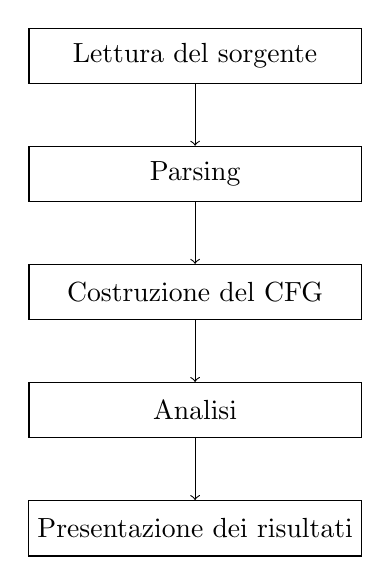
\begin{tikzpicture}[]
    
        \tikzstyle{block} = [draw, fill=white, rectangle, minimum height=2em, minimum width=12em]
    
        \node[block] (n1) at (0,10) {Lettura del sorgente};
        \node[block] (n2) at (0,8.5)  {Parsing};
        \node[block] (n3) at (0,7)  {Costruzione del CFG};
        \node[block] (n4) at (0,5.5)  {Analisi};
        \node[block] (n5) at (0,4)  {Presentazione dei risultati};
        
        \draw[->] (n1) -- (n2); 
        \draw[->] (n2) -- (n3); 
        \draw[->] (n3) -- (n4); 
        \draw[->] (n4) -- (n5);
    \end{tikzpicture}
\end{document}